\documentclass{article}

\def \lastexercisenumber {18}

% ---------------------------------------------------------------- %
% short package descriptions are copied from
% https://ctan.org/

% ---------------------------------------------------------------- %

% Accept different input encodings
\usepackage[utf8]{inputenc}

% Standard package for selecting font encodings
\usepackage[T1]{fontenc}

% ---------------------------------------------------------------- %

% Multilingual support for Plain TEX or LATEX
\usepackage[ngerman]{babel}

% ---------------------------------------------------------------- %

% Set all page margins to 1.5cm
\usepackage{fullpage}

% Margin adjustment and detection of odd/even pages
\usepackage{changepage}

% Flexible and complete interface to document dimensions
\usepackage{geometry}

% ---------------------------------------------------------------- %
% mathematics

\usepackage{amsmath}  % AMS mathematical facilities for LATEX
\usepackage{amssymb}
\usepackage{amsfonts} % TEX fonts from the American Mathematical Society
\usepackage{amsthm}   % Typesetting theorems (AMS style)

% Mathematical tools to use with amsmath
\usepackage{mathtools}

% Support for using RSFS fonts in maths
\usepackage{mathrsfs}

% Commands to produce dots in math that respect font size
\usepackage{mathdots}

% "Blackboard-style" cm fonts
\usepackage{bbm}

% Typeset in-line fractions in a "nice" way
\usepackage{nicefrac}

% Typeset quotient structures with LATEX
\usepackage{faktor}

% Vector arrows
\usepackage{esvect}

% St Mary Road symbols for theoretical computer science
\usepackage{stmaryrd}

% Three series of mathematical symbols
\usepackage{mathabx}

% ---------------------------------------------------------------- %
% algorithms

% Package for typesetting pseudocode
\usepackage{algpseudocode}

% Typeset source code listings using LATEX
\usepackage{listings}

% Reimplementation of and extensions to LATEX verbatim
\usepackage{verbatim}

% If necessary, please use the following 2 packages locally, but never both.
% This is because the algorithm environment gets defined in both packages, which leads to name conflicts.
% \usepackage{algorithm2e}
% \usepackage{algorithm}

% ---------------------------------------------------------------- %
% utilities

% A generic document command parser
\usepackage{xparse}

% Extended conditional commands
\usepackage{xifthen}

% e-TEX tools for LATEX
\usepackage{etoolbox}

% Define commands with suffixes
\usepackage{suffix}

% Extensive support for hypertext in LATEX
\usepackage{hyperref}

% Driver-independent color extensions for LATEX and pdfLATEX
\usepackage{xcolor}

% ---------------------------------------------------------------- %
% graphics

% -------------------------------- %

\usepackage{tikz}

% MISC
\usetikzlibrary{patterns}
\usetikzlibrary{decorations.markings}
\usetikzlibrary{positioning}
\usetikzlibrary{arrows}
\usetikzlibrary{arrows.meta}
\usetikzlibrary{overlay-beamer-styles}

% finite state machines
\usetikzlibrary{automata}

% turing machines
\usetikzlibrary{calc}
\usetikzlibrary{chains}
\usetikzlibrary{decorations.pathmorphing}

% -------------------------------- %

% Draw tree structures
\usepackage[noeepic]{qtree}

% Enhanced support for graphics
\usepackage{graphicx}

% Figures broken into subfigures
\usepackage{subfig}

% Improved interface for floating objects
\usepackage{float}

% Control float placement
\usepackage{placeins}

% Include PDF documents in LATEX
\usepackage{pdfpages}

% ---------------------------------------------------------------- %

% Control layout of itemize, enumerate, description
\usepackage[inline]{enumitem}

% Intermix single and multiple columns
\usepackage{multicol}
\setlength{\columnsep}{1cm}

% Coloured boxes, for LATEX examples and theorems, etc
\usepackage{tcolorbox}

% ---------------------------------------------------------------- %
% tables

% Tabulars with adjustable-width columns
\usepackage{tabularx}

% Tabular column heads and multilined cells
\usepackage{makecell}

% Publication quality tables in LATEX
\usepackage{booktabs}

% ---------------------------------------------------------------- %
% bibliography and quoting

% Sophisticated Bibliographies in LATEX
\usepackage[backend = biber, style = alphabetic]{biblatex}

% Context sensitive quotation facilities
\usepackage{csquotes}

% ---------------------------------------------------------------- %

% ---------------------------------------------------------------- %
% special letters

\newcommand{\N}{\mathbb N}
\newcommand{\Z}{\mathbb Z}
\newcommand{\Q}{\mathbb Q}
\newcommand{\R}{\mathbb R}
\newcommand{\C}{\mathbb C}
\newcommand{\K}{\mathbb K}
\newcommand{\T}{\mathbb T}
\newcommand{\E}{\mathbb E}
\newcommand{\V}{\mathbb V}
\renewcommand{\S}{\mathbb S}
\renewcommand{\P}{\mathbb P}
\newcommand{\1}{\mathbbm 1}
\newcommand{\G}{\mathbb G}

\newcommand{\iu}{\mathrm i}

% ---------------------------------------------------------------- %
% quantors

\newcommand{\Forall}        {\forall ~}
\newcommand{\Exists}        {\exists ~}
\newcommand{\nExists}       {\nexists ~}
\newcommand{\ExistsOnlyOne} {\exists! ~}
\newcommand{\nExistsOnlyOne}{\nexists! ~}
\newcommand{\ForAlmostAll}  {\forall^\infty ~}

% ---------------------------------------------------------------- %
% graphics boxed

\newcommand
{\includegraphicsboxed}
[2][0.75]
{
    \begin{center}
        \begin{tcolorbox}[standard jigsaw, opacityback = 0]

            \centering
            \includegraphics[width = #1 \textwidth]{#2}

        \end{tcolorbox}
    \end{center}
}

\newcommand
{\includegraphicsunboxed}
[2][0.75]
{
    \begin{center}
        \includegraphics[width = #1 \textwidth]{#2}
    \end{center}
}

\NewDocumentCommand
{\includegraphicsgraphicsboxed}
{ O{0.75} O{0.25} m m}
{
    \begin{center}
        \begin{tcolorbox}[standard jigsaw, opacityback = 0]

            \centering
            \includegraphics[width = #1 \textwidth]{#3} \\
            \vspace{#2 cm}
            \includegraphics[width = #1 \textwidth]{#4}

        \end{tcolorbox}
    \end{center}
}

\NewDocumentCommand
{\includegraphicsgraphicsunboxed}
{ O{0.75} O{0.25} m m}
{
    \begin{center}

        \centering
        \includegraphics[width = #1 \textwidth]{#3} \\
        \vspace{#2 cm}
        \includegraphics[width = #1 \textwidth]{#4}

    \end{center}
}

% ---------------------------------------------------------------- %
% braces

\newcommand{\pbraces}[1]{{\left  ( #1 \right  )}}
\newcommand{\bbraces}[1]{{\left  [ #1 \right  ]}}
\newcommand{\Bbraces}[1]{{\left \{ #1 \right \}}}
\newcommand{\vbraces}[1]{{\left  | #1 \right  |}}
\newcommand{\Vbraces}[1]{{\left \| #1 \right \|}}

\newcommand{\abraces}[1]{{\left \langle #1 \right \rangle}}

\newcommand{\floorbraces}[1]{{\left \lfloor #1 \right \rfloor}}
\newcommand{\ceilbraces} [1]{{\left \lceil  #1 \right \rceil }}

\newcommand{\dbbraces}    [1]{{\llbracket     #1 \rrbracket}}
\newcommand{\dpbraces}    [1]{{\llparenthesis #1 \rrparenthesis}}
\newcommand{\dfloorbraces}[1]{{\llfloor       #1 \rrfloor}}
\newcommand{\dceilbraces} [1]{{\llceil        #1 \rrceil}}

\newcommand{\dabraces}[1]{{\left \langle \left \langle #1 \right \rangle \right \rangle}}

\newcommand{\abs}  [1]{\vbraces{#1}}
\newcommand{\round}[1]{\bbraces{#1}}
\newcommand{\floor}[1]{\floorbraces{#1}}
\newcommand{\ceil} [1]{\ceilbraces{#1}}

% ---------------------------------------------------------------- %

% MISC

% metric spaces
\newcommand{\norm}[2][]{\Vbraces{#2}_{#1}}
\DeclareMathOperator{\metric}{d}
\DeclareMathOperator{\dist}  {dist}
\DeclareMathOperator{\diam}  {diam}

% O-notation
\newcommand{\landau}{{\scriptstyle \mathcal{O}}}
\newcommand{\Landau}{\mathcal{O}}

% ---------------------------------------------------------------- %

% math operators

% hyperbolic trigonometric function inverses
\DeclareMathOperator{\areasinh}{areasinh}
\DeclareMathOperator{\areacosh}{areacosh}
\DeclareMathOperator{\areatanh}{areatanh}

% special functions
\DeclareMathOperator{\id} {id}
\DeclareMathOperator{\sgn}{sgn}
\DeclareMathOperator{\Inv}{Inv}
\DeclareMathOperator{\erf}{erf}
\DeclareMathOperator{\pv} {pv}

% exponential function as power
\WithSuffix \newcommand \exp* [1]{\mathrm{e}^{#1}}

% operations on sets
\DeclareMathOperator{\meas}{meas}
\DeclareMathOperator{\card}{card}
\DeclareMathOperator{\Span}{span}
\DeclareMathOperator{\conv}{conv}
\DeclareMathOperator{\cof}{cof}
\DeclareMathOperator{\mean}{mean}
\DeclareMathOperator{\avg}{avg}
\DeclareMathOperator*{\argmax}{argmax}
\DeclareMathOperator*{\argsmax}{argsmax}

% number theory stuff
\DeclareMathOperator{\ggT}{ggT}
\DeclareMathOperator{\kgV}{kgV}
\DeclareMathOperator{\modulo}{mod}

% polynomial stuff
\DeclareMathOperator{\ord}{ord}
\DeclareMathOperator{\grad}{grad}

% function properties
\DeclareMathOperator{\ran}{ran}
\DeclareMathOperator{\supp}{supp}
\DeclareMathOperator{\graph}{graph}
\DeclareMathOperator{\dom}{dom}
\DeclareMathOperator{\Def}{def}
\DeclareMathOperator{\rg}{rg}

% matrix stuff
\DeclareMathOperator{\GL}{GL}
\DeclareMathOperator{\SL}{SL}
\DeclareMathOperator{\U}{U}
\DeclareMathOperator{\SU}{SU}
\DeclareMathOperator{\PSU}{PSU}
% \DeclareMathOperator{\O}{O}
% \DeclareMathOperator{\PO}{PO}
% \DeclareMathOperator{\PSO}{PSO}
\DeclareMathOperator{\diag}{diag}

% algebra stuff
\DeclareMathOperator{\At}{At}
\DeclareMathOperator{\Ob}{Ob}
\DeclareMathOperator{\Hom}{Hom}
\DeclareMathOperator{\End}{End}
\DeclareMathOperator{\Aut}{Aut}
\DeclareMathOperator{\Lin}{L}

% other function classes
\DeclareMathOperator{\Lip}{Lip}
\DeclareMathOperator{\Mod}{Mod}
\DeclareMathOperator{\Dil}{Dil}

% constants
\DeclareMathOperator{\NIL}{NIL}
\DeclareMathOperator{\eps}{eps}

% ---------------------------------------------------------------- %
% doubble & tripple powers

\newcommand
{\primeprime}
{{\prime \prime}}

\newcommand
{\primeprimeprime}
{{\prime \prime \prime}}

\newcommand
{\astast}
{{\ast \ast}}

\newcommand
{\astastast}
{{\ast \ast \ast}}

% ---------------------------------------------------------------- %
% derivatives

\NewDocumentCommand
{\derivative}
{ O{} O{} m m}
{
    \frac
    {\mathrm d^{#2} {#1}}
    {\mathrm d {#3}^{#2}}
}

\NewDocumentCommand
{\pderivative}
{ O{} O{} m m}
{
    \frac
    {\partial^{#2} {#1}}
    {\partial {#3}^{#2}}
}

\DeclareMathOperator{\Div}{div}
\DeclareMathOperator{\rot}{rot}

% ---------------------------------------------------------------- %
% integrals

\NewDocumentCommand
{\Int}
{ O{} O{} m m}
{\int_{#1}^{#2} #3 ~ \mathrm d #4}

\NewDocumentCommand
{\Iint}
{ O{} O{} m m m}
{\iint_{#1}^{#2} #3 ~ \mathrm d #4 ~ \mathrm d #5}

\NewDocumentCommand
{\Iiint}
{ O{} O{} m m m m}
{\iiint_{#1}^{#2} #3 ~ \mathrm d #4 ~ \mathrm d #5 ~ \mathrm d #6}

\NewDocumentCommand
{\Iiiint}
{ O{} O{} m m m m m}
{\iiiint_{#1}^{#2} #3 ~ \mathrm d #4 ~ \mathrm d #5 ~ \mathrm d #6 ~ \mathrm d #7}

\NewDocumentCommand
{\Idotsint}
{ O{} O{} m m m}
{\idotsint_{#1}^{#2} #3 ~ \mathrm d #4 \dots ~ \mathrm d #5}

\NewDocumentCommand
{\Oint}
{ O{} O{} m m}
{\oint_{#1}^{#2} #3 ~ \mathrm d #4}

% ---------------------------------------------------------------- %

% source:
% https://tex.stackexchange.com/questions/203257/tikz-chains-with-one-side-of-the-leftmost-node-thickbold

% #1 (optional): current state, e.g. $q_0$
% #2: cursor position, e.g. 1
% #3: number of displayed cells, e.g. 5
% #4: contents of cells, e.g. {$\triangleright$, $x_1$, \dots, $x_n$, \textvisiblespace}

\newcommand{\turingtape}[4][]
{
    \begin{tikzpicture}

        \tikzset{tape/.style={minimum size=.7cm, draw}}

        \begin{scope}[start chain=0 going right, node distance=0mm]
            \foreach \x [count=\i] in #4
            {
                \ifnum\i=#3 % if last node reset outer sep to 0pt
                    \node [on chain=0, tape, outer sep=0pt] (n\i) {\x};
                    \draw (n\i.north east) -- ++(.1,0) decorate [decoration={zigzag, segment length=.12cm, amplitude=.02cm}] {-- ($(n\i.south east)+(+.1,0)$)} -- (n\i.south east) -- cycle;
                \else
                    \node [on chain=0, tape] (n\i) {\x};
                \fi

                \ifnum\i=1 % if first node draw a thick line at the left
                    \draw [line width=.1cm] (n\i.north west) -- (n\i.south west);
                \fi
            }
 
            \node [right=.25cm of n#3] {$\cdots$};
            \node [tape, above left=.25cm and 1cm of n1] (q) {#1};
            \draw [>=latex, ->] (q) -| (n#2);

        \end{scope}

    \end{tikzpicture}
}

% ---------------------------------------------------------------- %

% ---------------------------------------------------------------- %
% amsthm-environments:

\theoremstyle{definition}

% numbered theorems
\newtheorem{theorem}             {Satz}[section]
\newtheorem{lemma}      [theorem]{Lemma}
\newtheorem{corollary}  [theorem]{Korollar}
\newtheorem{proposition}[theorem]{Proposition}
\newtheorem{remark}     [theorem]{Bemerkung}
\newtheorem{definition} [theorem]{Definition}
\newtheorem{example}    [theorem]{Beispiel}
\newtheorem{heuristics} [theorem]{Heuristik}

% unnumbered theorems
\newtheorem*{theorem*}    {Satz}
\newtheorem*{lemma*}      {Lemma}
\newtheorem*{corollary*}  {Korollar}
\newtheorem*{proposition*}{Proposition}
\newtheorem*{remark*}     {Bemerkung}
\newtheorem*{definition*} {Definition}
\newtheorem*{example*}    {Beispiel}
\newtheorem*{heuristics*} {Heuristik}

% ---------------------------------------------------------------- %
% exercise- and solution-environments:

% Please define this stuff in project ("main.tex"):
% \def \lastexercisenumber {...}

\newtheorem{exercise}{Aufgabe}
\setcounter{exercise}{\lastexercisenumber}

\newenvironment{solution}
{
  \begin{proof}[Lösung]
}{
  \end{proof}
}

% ---------------------------------------------------------------- %
% MISC translations for environment-names

\renewcommand{\proofname} {Beweis}
\renewcommand{\figurename}{Abbildung}
\renewcommand{\tablename} {Tabelle}

% ---------------------------------------------------------------- %

% ---------------------------------------------------------------- %
% https://www.overleaf.com/learn/latex/Code_listing

\definecolor{codegreen} {rgb}{0, 0.6, 0}
\definecolor{codegray}    {rgb}{0.5, 0.5, 0.5}
\definecolor{codepurple}{rgb}{0.58, 0, 0.82}
\definecolor{backcolour}{rgb}{0.95, 0.95, 0.92}

\lstdefinestyle{overleaf}
{
    backgroundcolor = \color{backcolour},
    commentstyle = \color{codegreen},
    keywordstyle = \color{magenta},
    numberstyle = \tiny\color{codegray},
    stringstyle = \color{codepurple},
    basicstyle = \ttfamily \footnotesize,
    breakatwhitespace = false,
    breaklines = true,
    captionpos = b,
    keepspaces = true,
    numbers = left,
    numbersep = 5pt,
    showspaces = false,
    showstringspaces = false,
    showtabs = false,
    tabsize = 2
}

% ---------------------------------------------------------------- %
% https://en.wikibooks.org/wiki/LaTeX/Source_Code_Listings

\lstdefinestyle{customc}
{
    belowcaptionskip = 1 \baselineskip,
    breaklines = true,
    frame = L,
    xleftmargin = \parindent,
    language = C,
    showstringspaces = false,
    basicstyle = \footnotesize \ttfamily,
    keywordstyle = \bfseries \color{green!40!black},
    commentstyle = \itshape \color{purple!40!black},
    identifierstyle = \color{blue},
    stringstyle = \color{orange},
}

\lstdefinestyle{customasm}
{
    belowcaptionskip = 1 \baselineskip,
    frame = L,
    xleftmargin = \parindent,
    language = [x86masm] Assembler,
    basicstyle = \footnotesize\ttfamily,
    commentstyle = \itshape\color{purple!40!black},
}

% ---------------------------------------------------------------- %
% https://tex.stackexchange.com/questions/235731/listings-syntax-for-literate

\definecolor{maroon}        {cmyk}{0, 0.87, 0.68, 0.32}
\definecolor{halfgray}      {gray}{0.55}
\definecolor{ipython_frame} {RGB}{207, 207, 207}
\definecolor{ipython_bg}    {RGB}{247, 247, 247}
\definecolor{ipython_red}   {RGB}{186, 33, 33}
\definecolor{ipython_green} {RGB}{0, 128, 0}
\definecolor{ipython_cyan}  {RGB}{64, 128, 128}
\definecolor{ipython_purple}{RGB}{170, 34, 255}

\lstdefinestyle{stackexchangePython}
{
    breaklines = true,
    %
    extendedchars = true,
    literate =
    {á}{{\' a}} 1 {é}{{\' e}} 1 {í}{{\' i}} 1 {ó}{{\' o}} 1 {ú}{{\' u}} 1
    {Á}{{\' A}} 1 {É}{{\' E}} 1 {Í}{{\' I}} 1 {Ó}{{\' O}} 1 {Ú}{{\' U}} 1
    {à}{{\` a}} 1 {è}{{\` e}} 1 {ì}{{\` i}} 1 {ò}{{\` o}} 1 {ù}{{\` u}} 1
    {À}{{\` A}} 1 {È}{{\' E}} 1 {Ì}{{\` I}} 1 {Ò}{{\` O}} 1 {Ù}{{\` U}} 1
    {ä}{{\" a}} 1 {ë}{{\" e}} 1 {ï}{{\" i}} 1 {ö}{{\" o}} 1 {ü}{{\" u}} 1
    {Ä}{{\" A}} 1 {Ë}{{\" E}} 1 {Ï}{{\" I}} 1 {Ö}{{\" O}} 1 {Ü}{{\" U}} 1
    {â}{{\^ a}} 1 {ê}{{\^ e}} 1 {î}{{\^ i}} 1 {ô}{{\^ o}} 1 {û}{{\^ u}} 1
    {Â}{{\^ A}} 1 {Ê}{{\^ E}} 1 {Î}{{\^ I}} 1 {Ô}{{\^ O}} 1 {Û}{{\^ U}} 1
    {œ}{{\oe}}  1 {Œ}{{\OE}}  1 {æ}{{\ae}}  1 {Æ}{{\AE}}  1 {ß}{{\ss}}  1
    {ç}{{\c c}} 1 {Ç}{{\c C}} 1 {ø}{{\o}} 1 {å}{{\r a}} 1 {Å}{{\r A}} 1
    {€}{{\EUR}} 1 {£}{{\pounds}} 1
}


% Python definition (c) 1998 Michael Weber
% Additional definitions (2013) Alexis Dimitriadis
% modified by me (should not have empty lines)

\lstdefinelanguage{iPython}{
    morekeywords = {access, and, break, class, continue, def, del, elif, else, except, exec, finally, for, from, global, if, import, in, is, lambda, not, or, pass, print, raise, return, try, while}, %
    %
    % Built-ins
    morekeywords = [2]{abs, all, any, basestring, bin, bool, bytearray, callable, chr, classmethod, cmp, compile, complex, delattr, dict, dir, divmod, enumerate, eval, execfile, file, filter, float, format, frozenset, getattr, globals, hasattr, hash, help, hex, id, input, int, isinstance, issubclass, iter, len, list, locals, long, map, max, memoryview, min, next, object, oct, open, ord, pow, property, range, raw_input, reduce, reload, repr, reversed, round, set, setattr, slice, sorted, staticmethod, str, sum, super, tuple, type, unichr, unicode, vars, xrange, zip, apply, buffer, coerce, intern}, %
    %
    sensitive = true, %
    morecomment = [l] \#, %
    morestring = [b]', %
    morestring = [b]", %
    %
    morestring = [s]{'''}{'''}, % used for documentation text (mulitiline strings)
    morestring = [s]{"""}{"""}, % added by Philipp Matthias Hahn
    %
    morestring = [s]{r'}{'},     % `raw' strings
    morestring = [s]{r"}{"},     %
    morestring = [s]{r'''}{'''}, %
    morestring = [s]{r"""}{"""}, %
    morestring = [s]{u'}{'},     % unicode strings
    morestring = [s]{u"}{"},     %
    morestring = [s]{u'''}{'''}, %
    morestring = [s]{u"""}{"""}, %
    %
    % {replace}{replacement}{lenght of replace}
    % *{-}{-}{1} will not replace in comments and so on
    literate = 
    {á}{{\' a}} 1 {é}{{\' e}} 1 {í}{{\' i}} 1 {ó}{{\' o}} 1 {ú}{{\' u}} 1
    {Á}{{\' A}} 1 {É}{{\' E}} 1 {Í}{{\' I}} 1 {Ó}{{\' O}} 1 {Ú}{{\' U}} 1
    {à}{{\` a}} 1 {è}{{\` e}} 1 {ì}{{\` i}} 1 {ò}{{\` o}} 1 {ù}{{\` u}} 1
    {À}{{\` A}} 1 {È}{{\' E}} 1 {Ì}{{\` I}} 1 {Ò}{{\` O}} 1 {Ù}{{\` U}} 1
    {ä}{{\" a}} 1 {ë}{{\" e}} 1 {ï}{{\" i}} 1 {ö}{{\" o}} 1 {ü}{{\" u}} 1
    {Ä}{{\" A}} 1 {Ë}{{\" E}} 1 {Ï}{{\" I}} 1 {Ö}{{\" O}} 1 {Ü}{{\" U}} 1
    {â}{{\^ a}} 1 {ê}{{\^ e}} 1 {î}{{\^ i}} 1 {ô}{{\^ o}} 1 {û}{{\^ u}} 1
    {Â}{{\^ A}} 1 {Ê}{{\^ E}} 1 {Î}{{\^ I}} 1 {Ô}{{\^ O}} 1 {Û}{{\^ U}} 1
    {œ}{{\oe}}  1 {Œ}{{\OE}}  1 {æ}{{\ae}}  1 {Æ}{{\AE}}  1 {ß}{{\ss}}  1
    {ç}{{\c c}} 1 {Ç}{{\c C}} 1 {ø}{{\o}} 1 {å}{{\r a}} 1 {Å}{{\r A}} 1
    {€}{{\EUR}} 1 {£}{{\pounds}} 1
    %
    {^}{{{\color{ipython_purple}\^ {}}}} 1
    { = }{{{\color{ipython_purple} = }}} 1
    %
    {+}{{{\color{ipython_purple}+}}} 1
    {*}{{{\color{ipython_purple}$^\ast$}}} 1
    {/}{{{\color{ipython_purple}/}}} 1
    %
    {+=}{{{+=}}} 1
    {-=}{{{-=}}} 1
    {*=}{{{$^\ast$ = }}} 1
    {/=}{{{/=}}} 1,
    literate = 
    *{-}{{{\color{ipython_purple} -}}} 1
     {?}{{{\color{ipython_purple} ?}}} 1,
    %
    identifierstyle = \color{black}\ttfamily,
    commentstyle = \color{ipython_cyan}\ttfamily,
    stringstyle = \color{ipython_red}\ttfamily,
    keepspaces = true,
    showspaces = false,
    showstringspaces = false,
    %
    rulecolor = \color{ipython_frame},
    frame = single,
    frameround = {t}{t}{t}{t},
    framexleftmargin = 6mm,
    numbers = left,
    numberstyle = \tiny\color{halfgray},
    %
    %
    backgroundcolor = \color{ipython_bg},
    % extendedchars = true,
    basicstyle = \scriptsize,
    keywordstyle = \color{ipython_green}\ttfamily,
}

% ---------------------------------------------------------------- %
% https://tex.stackexchange.com/questions/417884/colour-r-code-to-match-knitr-theme-using-listings-minted-or-other

\geometry{verbose, tmargin = 2.5cm, bmargin = 2.5cm, lmargin = 2.5cm, rmargin = 2.5cm}

\definecolor{backgroundCol}  {rgb}{.97, .97, .97}
\definecolor{commentstyleCol}{rgb}{0.678, 0.584, 0.686}
\definecolor{keywordstyleCol}{rgb}{0.737, 0.353, 0.396}
\definecolor{stringstyleCol} {rgb}{0.192, 0.494, 0.8}
\definecolor{NumCol}         {rgb}{0.686, 0.059, 0.569}
\definecolor{basicstyleCol}  {rgb}{0.345, 0.345, 0.345}

\lstdefinestyle{stackexchangeR}
{
    language = R,                                        % the language of the code
    basicstyle = \small \ttfamily \color{basicstyleCol}, % the size of the fonts that are used for the code
    % numbers = left,                                      % where to put the line-numbers
    numberstyle = \color{green},                         % the style that is used for the line-numbers
    stepnumber = 1,                                      % the step between two line-numbers. If it is 1, each line will be numbered
    numbersep = 5pt,                                     % how far the line-numbers are from the code
    backgroundcolor = \color{backgroundCol},             % choose the background color. You must add \usepackage{color}
    showspaces = false,                                  % show spaces adding particular underscores
    showstringspaces = false,                            % underline spaces within strings
    showtabs = false,                                    % show tabs within strings adding particular underscores
    % frame = single,                                      % adds a frame around the code
    % rulecolor = \color{white},                           % if not set, the frame-color may be changed on line-breaks within not-black text (e.g. commens (green here))
    tabsize = 2,                                         % sets default tabsize to 2 spaces
    captionpos = b,                                      % sets the caption-position to bottom
    breaklines = true,                                   % sets automatic line breaking
    breakatwhitespace = false,                           % sets if automatic breaks should only happen at whitespace
    keywordstyle = \color{keywordstyleCol},              % keyword style
    commentstyle = \color{commentstyleCol},              % comment style
    stringstyle = \color{stringstyleCol},                % string literal style
    literate = %
    *{0}{{{\color{NumCol} 0}}} 1
     {1}{{{\color{NumCol} 1}}} 1
     {2}{{{\color{NumCol} 2}}} 1
     {3}{{{\color{NumCol} 3}}} 1
     {4}{{{\color{NumCol} 4}}} 1
     {5}{{{\color{NumCol} 5}}} 1
     {6}{{{\color{NumCol} 6}}} 1
     {7}{{{\color{NumCol} 7}}} 1
     {8}{{{\color{NumCol} 8}}} 1
     {9}{{{\color{NumCol} 9}}} 1
}

% ---------------------------------------------------------------- %
% Fundament Mathematik

\lstdefinestyle{fundament}{basicstyle = \ttfamily}

% ---------------------------------------------------------------- %


\addbibresource{../../../Fundament-LaTeX/references.bib}

\graphicspath{{../../../Fundament-LaTeX/images/}}

\parskip 0pt
\parindent 0pt

\title
{
  Diskrete und Geometrische Algorithmen \\
  \vspace{4pt}
  \normalsize
  \textit{4. Übung am 16.11.2020}
}
\author
{
  Richard Weiss
  \and
  Florian Schager
  \and
  Christian Sallinger
  \and
  Fabian Zehetgruber
  \and
  Paul Winkler
  \and
  Christian Göth
}
\date{}

\begin{document}

\maketitle

% --------------------------------------------------------------------------------

\begin{exercise}

Für ein beschränktes Lipschitz-Gebiet $\Omega \subset \R^2$ definieren wir den Hilbertraum

\begin{align*}
  H(\curl, \Omega)
  :=
  \Bbraces{\xi \in [L^2(\Omega)]^2 | \curl \xi \in L^2(\Omega)}, 
  \quad
  (\xi, \zeta)_{H(\curl)}
  :=
  (\xi, \zeta)_{L^2(\Omega)} + (\curl \xi, \curl \zeta)_{L^2(\Omega)}, 
\end{align*}

mit $\curl \xi := \frac{\partial \xi_2}{\partial x} - \frac{\partial \xi_1}{\partial y}$ für $\xi(x, y) = (\xi_1(x, y), \xi_2(x, y))^\top$.
Weiter sei $X := H^1_0(\Omega) \times H(\curl, \Omega)$ ein Hilbert-Raum wie in Aufgabe 6.

Für ein $c \geq 0$ und $f \in L^2(\Omega)$ sei das folgende Variationsproblem gegeben: Finden Sie $(u, \xi) \in X$ sodass für alle $(v, \zeta) \in X$

\begin{align}
  \Int[\Omega]{(\nabla u - \xi) \cdot (\nabla v - \zeta)}{x}
  +
  c \Int[\Omega]{\xi \cdot \zeta}{x}
  +
  \Int[\Omega]{\curl \xi \curl \zeta}{x}
  =
  \Int[\Omega]{f v}{x}
\end{align}

\begin{enumerate}[label = \textbf{\alph*)}]

  \item Zeigen Sie mit Hilfe des Lemmas von Lax-Milgram, dass für $c > 0$ das Problem eine eindeutige Lösung hat.
  Verwenden Sie dazu am besten die Young Ungleichung $-ab \geq - \frac{\varepsilon}{2} a^2 - \frac{1}{2\varepsilon}b^2$ für geeignete $a, b \in \R$ und $\varepsilon > 0$.

  \item Es sei nun $c = 0$.
  Zeigen Sie durch geschicktes Wählen von $(u, \xi) \in X$, dass das Problem nicht koerziv ist.
  \textit{Hinweis}:
  Was gilt für $\curl \nabla u$?

  \item Begründen Sie mit den Funktionen $\xi_\varepsilon \in [H^1(\Omega)]^2$ definiert durch $\xi_\varepsilon(x, y) := (\sin(\frac{1}{\varepsilon}x), 0)^\top$ mit $\varepsilon > 0$, dass das Problem auf dem Produktraum $\hat{X} := H^1_0(\Omega) \times [H^1(\Omega)]^2$ mit $c > 0$ nicht koerziv und damit nicht wohlgestellt ist.

\end{enumerate}

\end{exercise}

% --------------------------------------------------------------------------------

\begin{solution}

\phantom{}

\begin{align*}
  \pbraces
  {
    \begin{pmatrix}
      u \\ \xi
    \end{pmatrix},
    \begin{pmatrix}
      v \\ \zeta
    \end{pmatrix}
  }_X
  & =
  (u, v)_{H^1(\Omega)}
  +
  (\xi, \zeta)_{H(\curl, \Omega)} \\
  & =
  (u, v)_{L^2(\Omega)}
  +
  (\nabla u, \nabla v)_{L^2(\Omega)}
  +
  (\xi, \zeta)_{L^2(\Omega)}
  +
  (\curl \xi, \curl \zeta)_{L^2(\Omega)}
\end{align*}

\begin{align*}
  \implies
  \norm[X]
  {
    \begin{pmatrix}
      u \\ \xi
    \end{pmatrix}
  }
  & =
  \pbraces
  {
    \begin{pmatrix}
      u \\ \xi
    \end{pmatrix},
    \begin{pmatrix}
      u \\ \xi
    \end{pmatrix}
  }_X^{1/2} \\
  & =
  \pbraces
  {
    (u, u)_{L^2(\Omega)}
    +
    (\nabla u, \nabla u)_{L^2(\Omega)}
    +
    (\xi, \xi)_{L^2(\Omega)}
    +
    (\curl \xi, \curl \xi)_{L^2(\Omega)}
  }^{1/2} \\
  & =
  \pbraces
  {
    \norm[L^2(\Omega)]{u}^2
    +
    \norm[L^2(\Omega)]{\nabla u}^2
    +
    \norm[L^2(\Omega)]{\xi}^2
    +
    \norm[L^2(\Omega)]{\curl \xi}^2
  }^{1/2}
\end{align*}

\begin{enumerate}[label = \textbf{\alph*)}]

  \item \phantom{}

  \begin{center}
    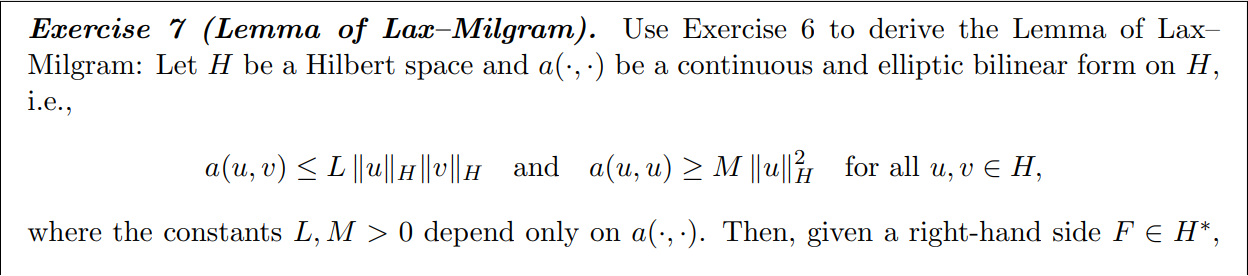
\includegraphics[width = 0.75 \textwidth]{NumPDEs/NumPDEs - Exercise 7.1 (Lemma of Lax-Milgram).png} \\
    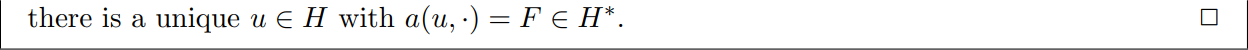
\includegraphics[width = 0.75 \textwidth]{NumPDEs/NumPDEs - Exercise 7.2 (Lemma of Lax-Milgram).png}
  \end{center}

  \begin{align*}
    a
    \pbraces
    {
      \begin{pmatrix}
        u \\ \xi
      \end{pmatrix},
      \begin{pmatrix}
        v \\ \zeta
      \end{pmatrix}
    }
    & :=
    \Int[\Omega]{(\nabla u - \xi) \cdot (\nabla v - \zeta)}{x}
    +
    c \Int[\Omega]{\xi \cdot \zeta}{x}
    +
    \Int[\Omega]{\curl \xi \curl \zeta}{x} \\
    F
    \begin{pmatrix}
      v \\ \xi
    \end{pmatrix}
    & :=
    \Int[\Omega]{f v}{x}
  \end{align*}

  \begin{enumerate}[label = \arabic*.]

    \item Stetigkeit von $a$:
    
    Auf dem $\R^3$ sind die Normen $\norm[1]{\cdot}$ und $\norm[2]{\cdot}$ äquivalent.
    Wir erhalten also eine Konstante $C > 0$, sodass $\norm[1]{\cdot} \leq C \norm[2]{\cdot}$.

    \begin{align*}
      \norm[1]{\cdot}
      \sim
      \norm[2]{\cdot}
      ~\text{auf $\R^3$}~
      \implies
      \Exists C > 0:
      \norm[1]{\cdot}
      \leq
      C
      \norm[2]{\cdot}
    \end{align*}

    \begin{align*}
      a
      \pbraces
      {
        \begin{pmatrix}
          u \\ \xi
        \end{pmatrix},
        \begin{pmatrix}
          v \\ \zeta
        \end{pmatrix}
      }
      & =
      \Int[\Omega]{(\nabla u - \xi) \cdot (\nabla v - \zeta)}{x}
      +
      c \Int[\Omega]{\xi \cdot \zeta}{x}
      +
      \Int[\Omega]{\curl \xi \curl \zeta}{x} \\
      & \stackrel
      {
        \mathrm{CSB}
      }{\leq}
      \norm[L^2(\Omega)]{\nabla u - \xi}
      \norm[L^2(\Omega)]{\nabla v - \zeta} \\
      & \quad
      +
      c
      \norm[L^2(\Omega)]{\xi}
      \norm[L^2(\Omega)]{\zeta}
      +
      \norm[L^2(\Omega)]{\curl \xi}
      \norm[L^2(\Omega)]{\curl \zeta} \\
      & \leq
      \pbraces
      {
        \norm[L^2(\Omega)]{\nabla u}
        +
        \norm[L^2(\Omega)]{\xi}
      }
      \pbraces
      {
        \norm[L^2(\Omega)]{\nabla u}
        +
        \norm[L^2(\Omega)]{\zeta}
      } \\
      & \quad
      +
      c
      \norm[L^2(\Omega)]{\xi}
      \norm[L^2(\Omega)]{\zeta}
      +
      \norm[L^2(\Omega)]{\curl \xi}
      \norm[L^2(\Omega)]{\curl \zeta} \\
      & \leq
      2 \max \Bbraces{1, c} \\
      & \quad
      \pbraces
      {
        \norm[H^1(\Omega)]{u}
        +
        \norm[L^2(\Omega)]{\xi}
        +
        \norm[L^2(\Omega)]{\curl \xi}
      } \\
      & \quad
      \pbraces
      {
        \norm[H^1(\Omega)]{v}
        +
        \norm[L^2(\Omega)]{\zeta}
        +
        \norm[L^2(\Omega)]{\curl \zeta}
      } \\
      & =
      2 \max \Bbraces{1, c} \\
      & \quad
      \norm[1]
      {
        \pbraces
        {
          \norm[H^1(\Omega)]{u},
          \norm[L^2(\Omega)]{\xi},
          \norm[L^2(\Omega)]{\curl \xi}
        }^\top
      } \\
      & \quad
      \norm[1]
      {
        \pbraces
        {
          \norm[H^1(\Omega)]{v},
          \norm[L^2(\Omega)]{\zeta},
          \norm[L^2(\Omega)]{\curl \zeta}
        }^\top
      } \\
      & \leq
      2 \max \Bbraces{1, c} C^2 \\
      & \quad
      \norm[2]
      {
        \pbraces
        {
          \norm[H^1(\Omega)]{u},
          \norm[L^2(\Omega)]{\xi},
          \norm[L^2(\Omega)]{\curl \xi}
        }^\top
      } \\
      & \quad
      \norm[2]
      {
        \pbraces
        {
          \norm[H^1(\Omega)]{v},
          \norm[L^2(\Omega)]{\zeta},
          \norm[L^2(\Omega)]{\curl \zeta}
        }^\top
      } \\
      & =
      2 \max \Bbraces{1, c} C^2 \\
      & \quad
      \pbraces
      {
        \norm[H^1(\Omega)]{u}^2
        +
        \norm[L^2(\Omega)]{\xi}^2
        +
        \norm[L^2(\Omega)]{\curl \xi}^2
      }^{1/2} \\
      & \quad
      \pbraces
      {
        \norm[H^1(\Omega)]{v}^2
        +
        \norm[L^2(\Omega)]{\zeta}^2
        +
        \norm[L^2(\Omega)]{\curl \zeta}^2
      }^{1/2} \\
      & =
      2 \max \Bbraces{1, c} C^2
      \norm[X]
      {
        \begin{pmatrix}
          u \\ \xi
        \end{pmatrix}
      }
      \norm[X]
      {
        \begin{pmatrix}
          v \\ \zeta
        \end{pmatrix}
      }
    \end{align*}

    \item Elliptizität von $a$:
    
    \includegraphicsunboxed{PDEs/PDEs_-_Satz_5-11_(Poincare-Ungleichung).png}

    Die Poincaré-Ungleichung von \cite{PDEs} liefert uns ein $C_p > 0:$

    \begin{align*}
      \norm[H^1(\Omega)]{u}^2
      =
      \norm[L^2(\Omega)]{u}^2
      +
      \norm[L^2(\Omega)]{\nabla u}^2
      \leq
      (C_p + 1)^2 \norm[L^2(\Omega)]{\nabla u}^2
      \implies
      \norm[L^2(\Omega)]{\nabla u}
      \geq
      \frac{1}{C_p + 1}
      \norm[H^1(\Omega)]{u}^2.
    \end{align*}

    In der folgenden Abschätzung verwenden wir die Young Ungleichung mit $\varepsilon \in \pbraces{\frac{1}{c + 1}, 1}$.
    
    \begin{align*}
      a
      \pbraces
      {
        \begin{pmatrix}
          u \\ \xi
        \end{pmatrix},
        \begin{pmatrix}
          u \\ \xi
        \end{pmatrix}
      }
      & =
      \Int[\Omega]{(\nabla u - \xi) \cdot (\nabla u - \xi)}{x}
      +
      c \Int[\Omega]{\xi \cdot \xi}{x}
      +
      \Int[\Omega]{\curl \xi \curl \xi}{x} \\
      & =
      \norm[L^2(\Omega)]{\nabla u - \xi}^2
      +
      c \norm[L^2(\Omega)]{\xi}^2
      +
      \norm[L^2(\Omega)]{\curl \xi}^2 \\
      & \geq
      \pbraces
      {
        \norm[L^2(\Omega)]{\nabla u}
        -
        \norm[L^2(\Omega)]{\xi}
      }^2
      +
      c \norm[L^2(\Omega)]{\xi}^2
      +
      \norm[L^2(\Omega)]{\curl \xi}^2 \\
      & =
      \norm[L^2(\Omega)]{\nabla u}^2
      -
      2
      \norm[L^2(\Omega)]{\nabla u}
      \norm[L^2(\Omega)]{\xi}
      +
      \norm[L^2(\Omega)]{\xi}^2
      +
      c
      \norm[L^2(\Omega)]{\xi}^2
      +
      \norm[L^2(\Omega)]{\curl \xi}^2 \\
      & \stackrel
      {
        \mathrm{Y}
      }{\geq}
      \norm[L^2(\Omega)]{\nabla u}^2
      -
      \varepsilon
      \norm[L^2(\Omega)]{\nabla u}^2
      -
      \frac{1}{\varepsilon}
      \norm[L^2(\Omega)]{\xi}^2
      +
      \norm[L^2(\Omega)]{\xi}^2
      +
      c
      \norm[L^2(\Omega)]{\xi}^2
      +
      \norm[L^2(\Omega)]{\curl \xi}^2 \\
      & =
      (1 - \varepsilon)
      \norm[L^2(\Omega)]{\nabla u}^2
      +
      \pbraces{1 + c - \frac{1}{\varepsilon}}
      \norm[L^2(\Omega)]{\xi}^2
      +
      \norm[L^2(\Omega)]{\curl \xi}^2 \\
      & \geq
      \frac{1 - \varepsilon}{(C_p + 1)^2}
      \norm[H^1(\Omega)]{\nabla u}^2
      +
      \pbraces{1 + c - \frac{1}{\varepsilon}}
      \norm[L^2(\Omega)]{\xi}^2
      +
      \norm[L^2(\Omega)]{\curl \xi}^2 \\
      & \geq
      \min
      \Bbraces
      {
        \frac{1 - \varepsilon}{(C_p + 1)^2},
        1 + c - \frac{1}{\varepsilon},
        1
      }
      \pbraces
      {
        \norm[H^1(\Omega)]{\nabla u}^2
        +
        \norm[L^2(\Omega)]{\xi}^2
        +
        \norm[L^2(\Omega)]{\curl \xi}^2
      } \\
      & =
      \min
      \Bbraces
      {
        \frac{1 - \varepsilon}{(C_p + 1)^2},
        1 + c - \frac{1}{\varepsilon},
        1
      }
      \norm[X]
      {
        \begin{pmatrix}
          u \\ \xi
        \end{pmatrix}
      }^2
    \end{align*}

    Wir sind fertig, weil $c > 0$.

    \item Stetigkeit von $F$:
    
    \begin{align*}
      F
    \begin{pmatrix}
      v \\ \xi
    \end{pmatrix}
    =
    \Int[\Omega]{f v}{x}
    \stackrel
    {
      \mathrm{CSB}
    }{\leq}
    \norm[L^2(\Omega)]{f}
    \norm[L^2(\Omega)]{v}
    \leq
    \norm[L^2(\Omega)]{f}
    \norm[X]
    {
      \begin{pmatrix}
        v \\ \xi
      \end{pmatrix}  
    }
    \end{align*}

  \end{enumerate}

\end{enumerate}

\end{solution}

% --------------------------------------------------------------------------------

% --------------------------------------------------------------------------------

\begin{exercise}

\phantom{}

\begin{enumerate}[label = \textbf{\alph*)}]

  \item Es sei $\Omega = (0,1), t >0, f \in L^2(\Omega)$, und $X := H^1_D(\Omega) \times H^1_D(\Omega)$ mit $H^1_D(\Omega) := \Bbraces{u \in H^1(\Omega) | u(0) = 0}$.
  Das Problem des Timoshenko Balkens lautet:
  Gesucht ist $(w, \beta) \in X$ sodass für alle $(v, \delta) \in X$

  \begin{align}
    \Int[\Omega]{\beta^\prime \delta^\prime}{x}
    +
    \frac{1}{t^2} \Int[\Omega]{(w^\prime - \beta)(v^\prime - \delta)}{x}
    =
    \Int[\Omega]{f v}{x}.
  \end{align}

  Zeigen Sie, dass das Problem eindeutig lösbar ist. Wie verhält sich die Konstante in Cea's Lemma wenn $t \to 0$?
  \textit{Hinweis}:
  Verwenden Sie wie in Aufgabe 19 die Young Ungleichung für den gemischten Term sowie die Friedrich Ungleichung.

  \item Sei nun $\Omega \subset \R^2$ und $X := H^1_D(\Omega) \times [H^1_D(\Omega)]^2$.
  Betrachten Sie die Reissner-Mindlin Platte als zweidimiensionale Erweiterung des Timoshenko Balkens beschrieben durch das Problem:
  Gesucht ist $(w, \beta) \in X$ sodass für alle $(v, \delta) \in X$

  \begin{align}
    \Int[\Omega]{\epsilon(\beta):\epsilon(\delta)}{x}
    +
    \frac{1}{t^2} \Int[\Omega]{(\nabla w - \beta) \cdot (\nabla v - \delta)}{x}
    =
    \Int[\Omega]{f v}{x},
  \end{align}

  wobei $\epsilon(\beta) := 0.5 (\nabla \beta + (\nabla \beta)^\top)$ der symmetrische Gradient ist.
  Untersuchen Sie mit dem zur Verfügung gestellten Jupyter-File das Konvergenzverhalten für lineare Elemente bei verschiedenen Dickenparametern, $t \in \Bbraces{1, 0.1, 0.01, 0.001}$.
  Was beobachten Sie?
  Wie ändert sich das Verhalten für quadratisch finite Elemente?

\end{enumerate}

\end{exercise}

% --------------------------------------------------------------------------------

\begin{solution}

\phantom{}

\begin{enumerate}[label = \textbf{\alph*)}]

  \item Wir wollen wieder Exercise 7 (Lemma of Lax-Milgram) anwenden, diesmal mit

  \begin{align*}
    a
    \pbraces
    {
      \begin{pmatrix}
        w \\ \beta
      \end{pmatrix},
      \begin{pmatrix}
        v \\ \xi
      \end{pmatrix}
    }
    :=
    \Int[\Omega]{\beta^\prime \delta^\prime}{x}
    +
    \frac{1}{t^2} \Int[\Omega]{(w^\prime - \beta)(v^\prime - \delta)}{x},
    \quad
    F
    \begin{pmatrix}
      v \\ \delta
    \end{pmatrix}
    :=
    \Int[\Omega]{f v}{x}.
  \end{align*}

  \begin{enumerate}[label = \arabic*.]

    \item Schritt (Stetigkeit von $a$):
    
    Auf dem $\R^2$ sind die Normen $\norm[1]{\cdot}$ und $\norm[2]{\cdot}$ äquivalent.
    Wir erhalten also eine Konstante $C > 0$, sodass $\norm[1]{\cdot} \leq C \norm[2]{\cdot}$.

    \begin{align*}
      \norm[1]{\cdot}
      \sim
      \norm[2]{\cdot}
      ~\text{auf $\R^2$}~
      \implies
      \Exists C > 0:
      \norm[1]{\cdot}
      \leq
      C
      \norm[2]{\cdot}
    \end{align*}

    Vorausschauend auf das Lemma 1.6 (Céa), definieren wir noch die Konstante

    \begin{align*}
      \beta_t
      :=
      2 \max \Bbraces{1, \frac{1}{t^2}} C.
    \end{align*}

    \begin{align*}
      a
      \pbraces
      {
        \begin{pmatrix}
          w \\ \beta
        \end{pmatrix},
        \begin{pmatrix}
          v \\ \xi
        \end{pmatrix}
      }
      & =
      \Int[\Omega]{\beta^\prime \delta^\prime}{x}
      +
      \frac{1}{t^2} \Int[\Omega]{(w^\prime - \beta)(v^\prime - \delta)}{x} \\
      & \stackrel
      {
        \mathrm{CSB}
      }{\leq}
      \norm[L^2(\Omega)]{\beta^\prime}
      \norm[L^2(\Omega)]{\delta^\prime}
      +
      \frac{1}{t^2}
      \norm[L^2(\Omega)]{w^\prime - \beta}
      \norm[L^2(\Omega)]{v^\prime - \delta} \\
      & \leq
      \norm[L^2(\Omega)]{\beta^\prime}
      \norm[L^2(\Omega)]{\delta^\prime}
      +
      \frac{1}{t^2}
      \pbraces
      {
        \norm[L^2(\Omega)]{w^\prime}
        \norm[L^2(\Omega)]{\beta}
      }
      \pbraces
      {
        \norm[L^2(\Omega)]{v^\prime}
        \norm[L^2(\Omega)]{\delta}
      } \\
      & \leq
      2 \max \Bbraces{1, \frac{1}{t^2}}
      \pbraces
      {
        \norm[L^2(\Omega)]{w^\prime}
        \norm[L^2(\Omega)]{\beta}
      }
      \pbraces
      {
        \norm[L^2(\Omega)]{v^\prime}
        \norm[L^2(\Omega)]{\delta}
      } \\
      & = \cdots \leq
      2 \max \Bbraces{1, \frac{1}{t^2}} C
      \pbraces
      {
        \norm[L^2(\Omega)]{w^\prime}^2
        \norm[L^2(\Omega)]{\beta}^2
      }^{1/2}
      \pbraces
      {
        \norm[L^2(\Omega)]{v^\prime}^2
        \norm[L^2(\Omega)]{\delta}^2
      }^{1/2} \\
      & =
      \beta_t
      \norm[X]
      {
        \begin{pmatrix}
          w \\ \beta
        \end{pmatrix}
      }
      \norm[X]
      {
        \begin{pmatrix}
          v \\ \delta
        \end{pmatrix}
      }
    \end{align*}

    \item Schritt (Elliptizität von $a$):
    
    \begin{enumerate}[label = \arabic*.]

      \item Hilfs-Ungleichung (Friedrich):

      \begin{center}
        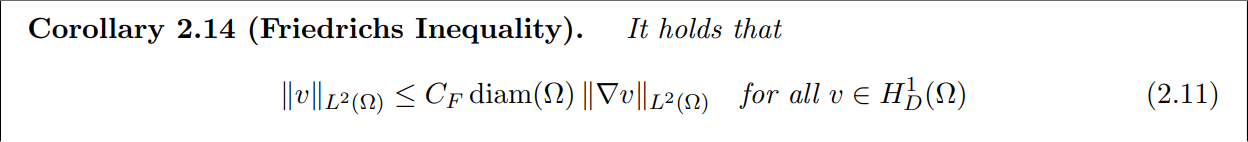
\includegraphics[width = 0.75 \textwidth]{NumPDEs/NumPDEs - Corollary 2.14.1 (Friedrichs Inequality).png} \\
        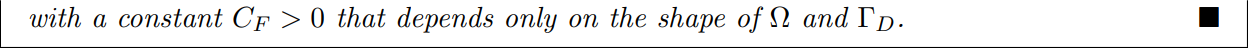
\includegraphics[width = 0.75 \textwidth]{NumPDEs/NumPDEs - Corollary 2.14.2 (Friedrichs Inequality).png}
      \end{center}

      \begin{align*}
        \implies
        \norm[H^1(\Omega)]{v}^2
        =
        \norm[L^2(\Omega)]{v}
        +
        \norm[L^2(\Omega)]{\nabla v}
        \stackrel
        {
          \mathrm{F}
        }{\leq}
        (
          C_F
          \underbrace{\diam \Omega}_1
          +
          1
        )^2
        \norm[L^2(\Omega)]{v^\prime}^2
      \end{align*}

      \item Hilfs-Ungleichung (Young):
      
      Dabei wollen wir $\varepsilon_t$ wie folgt wählen.

      \begin{align*}
        \varepsilon_t
        \in
        \pbraces
        {
          \frac{1}
          {
            1
            +
            \frac{t^2}{(C_F + 1)^2}
          },
          1
        }
        \neq
        \emptyset
      \end{align*}

      Das Intervall ist dabei nicht die leere Menge, weil $t > 0$ und daher

      \begin{align*}
        1 < 1 + \frac{t^2}{(C_F + 1)^2}.
      \end{align*}

    \end{enumerate}

    Vorausschauend auf das Lemma 1.6 (Céa), definieren wir noch die Konstante

    \begin{align*}
      \alpha_t
      :=
      \min
      \Bbraces
      {
        \frac{1}{(C_F + 1)^2}
        +
        \frac{1}{t^2}
        \pbraces
        {
          1 - \frac{1}{\varepsilon_t}
        },
        \frac
        {
          1 - \varepsilon_t
        }{
          t^2 (C_F + 1)^2
        }
      }.
    \end{align*}

    \begin{align*}
      a
      \pbraces
      {
        \begin{pmatrix}
          w \\ \beta
        \end{pmatrix},
        \begin{pmatrix}
          w \\ \beta
        \end{pmatrix}
      }
      & =
      \norm[L^2(\Omega)]{\beta^\prime}^2
      +
      \frac{1}{t^2}
      \Int[\Omega]{\abs{w^\prime - \beta}^2}{x} \\
      & =
      \norm[L^2(\Omega)]{\beta^\prime}^2
      +
      \frac{1}{t^2}
      \pbraces
      {
        \norm[L^2(\Omega)]{w^\prime}^2
        +
        \Int[\Omega]{- 2 w^\prime \beta}{x}
        +
        \norm[L^2(\Omega)]{\beta}^2
      } \\
      & \stackrel
      {
        \mathrm{Y}
      }{\geq}
      \norm[L^2(\Omega)]{\beta^\prime}^2
      +
      \frac{1}{t^2}
      \pbraces
      {
        \norm[L^2(\Omega)]{w^\prime}^2
        +
        \Int[\Omega]{- \varepsilon_t \abs{w^\prime}^2}{x}
        +
        \Int[\Omega]{- \frac{1}{\varepsilon_t} \abs{\beta}^2}{x}
        +
        \norm[L^2(\Omega)]{\beta}^2
      } \\
      & =
      \norm[L^2(\Omega)]{\beta^\prime}^2
      +
      \frac{1}{t^2}
      \pbraces
      {
        (1 - \varepsilon_t)
        \norm[L^2(\Omega)]{w^\prime}^2
        +
        \pbraces
        {
          1 - \frac{1}{\varepsilon_t}
        }
        \norm[L^2(\Omega)]{\beta}^2
      } \\
      & \stackrel
      {
        \mathrm{F}
      }{\geq}
      \frac{1}{(C_F + 1)^2}
      \norm[H^2(\Omega)]{\beta}^2
      +
      \frac{1}{t}
      \pbraces
      {
        \frac{1 - \varepsilon_t}{(C_F + 1)^2}
        \norm[H^1(\Omega)]{w}^2
        +
        \pbraces
        {
          1 - \frac{1}{\varepsilon_t}
        }
        \norm[H^1(\Omega)]{\beta}^2
      } \\
      & =
      \pbraces
      {
        \frac{1}{(C_F + 1)^2}
        +
        \frac{1}{t^2}
        \pbraces
        {
          1 - \frac{1}{\varepsilon_t}
        }
      }
      \norm[H^1(\Omega)]{\beta}^2
      +
      \frac{1 - \varepsilon_t}{t^2 (C_F + 1)^2}
      \norm[H^1(\Omega)]{w}^2 \\
      & \geq
      \min
      \Bbraces
      {
        \frac{1}{(C_F + 1)^2}
        +
        \frac{1}{t^2}
        \pbraces
        {
          1 - \frac{1}{\varepsilon_t}
        },
        \frac
        {
          1 - \varepsilon_t
        }{
          t^2 (C_F + 1)^2
        }
      }
      \pbraces
      {
        \norm[H^1(\Omega)]{w}^2
        +
        \norm[H^1(\Omega)]{\beta}^2
      } \\
      & =
      \alpha_t
      \norm[X]
      {
        \begin{pmatrix}
          w \\ \beta
        \end{pmatrix}
      }^2
    \end{align*}

    \item Schritt (Stetigkeit von $F$):
    
    \begin{align*}
      F
      \begin{pmatrix}
        v \\ \delta
      \end{pmatrix}
      =
      \Int[\Omega]{f v}{x}
      \stackrel
      {
        \mathrm{CSB}
      }{\leq}
      \norm[L^2(\Omega)]{f}
      \norm[L^2(\Omega)]{v}
      \leq
      \norm[L^2(\Omega)]{f}
      \norm[X]
      {
        \begin{pmatrix}
          v \\ \delta
        \end{pmatrix}
      }
    \end{align*}

  \end{enumerate}

  \includegraphicsunboxed{NumPDEs/NumPDEs - Lemma 1.6 (Céa).png}

  Der Quotient in Lemma 1.6 (Céa) divergiert.

  \begin{align*}
    \beta_t
    & =
    2 \max \Bbraces{1, \frac{1}{t^2}} C
    \xrightarrow{t \to 0}
    \infty, \\
    \alpha_t
    & =
    \min
    \Bbraces
    {
      \frac{1}{(C_F + 1)^2}
      +
      \frac{1}{t^2}
      \pbraces
      {
        1 - \frac{1}{\varepsilon_t}
      },
      \frac
      {
        1 - \varepsilon_t
      }{
        t^2 (C_F + 1)^2
      }
    }
    \leq
    \frac
    {
      1 - \varepsilon_t
    }{
      t^2 (C_F + 1)^2
    }
    \leq
    \frac
    {
      1
      -
      \frac{1}
      {
        1
        +
        \frac{t^2}{(C_F + 1)^2}
      }
    }{
      t^2 (C_F + 1)^2
    } \\
    & =
    \frac
    {
      1 + \frac{t^2}{(C_f + 1)^2} - 1
    }{
      \pbraces
      {
        1 + \frac{t^2}{(C_F + 1)^2}
      }
      t^2 (C_F + 1)^2
    }
    =
    \frac{1}
    {
      (C_F + 1)^2
      \pbraces
      {
        (C_F + 1)^2 + t^2
      }
    }
    \xrightarrow{t \to 0}
    \frac{1}{(C_F + 1)^4} \\
    \implies
    \frac{\beta_t}{\alpha_t}
    & \xrightarrow{t \to 0}
    \infty
  \end{align*}

  Die Fehlerschranke (d.h. die rechte Seite von (1.20)) kann also beliebig groß werden.
  Somit können wir Lemma 1.6 (Céa) nicht anwenden, um den FEM-Fehler sinnvoll abzuschätzen.

\end{enumerate}

\end{solution}

% --------------------------------------------------------------------------------

% -------------------------------------------------------------------------------- %

\begin{exercise}

ToDo!

\end{exercise}

% -------------------------------------------------------------------------------- %

\begin{solution}

ToDo!

\end{solution}

% -------------------------------------------------------------------------------- %

% -------------------------------------------------------------------------------- %

\begin{exercise}

ToDo!

\end{exercise}

% -------------------------------------------------------------------------------- %

\begin{solution}

ToDo!

\end{solution}

% -------------------------------------------------------------------------------- %

% -------------------------------------------------------------------------------- %

\begin{exercise}

ToDo!

\end{exercise}

% -------------------------------------------------------------------------------- %

\begin{solution}

ToDo!

\end{solution}

% -------------------------------------------------------------------------------- %

% -------------------------------------------------------------------------------- %

\begin{exercise}

ToDo!

\end{exercise}

% -------------------------------------------------------------------------------- %

\begin{solution}

ToDo!

\end{solution}

% -------------------------------------------------------------------------------- %


\printbibliography

\end{document}
